%\documentclass[german,10pt]{book}      
\usepackage{makeidx}
\usepackage{babel}            % Sprachunterstuetzung
\usepackage{amsmath}          % AMS "Grundpaket"
\usepackage{amssymb,amsfonts,amsthm,amscd} 
\usepackage{mathrsfs}
\usepackage{rotating}
\usepackage{sidecap}
\usepackage{graphicx}
\usepackage{color}
\usepackage{fancybox}
\usepackage{tikz}
\usetikzlibrary{arrows,snakes,backgrounds}
\usepackage{hyperref}
\hypersetup{colorlinks=true,
                    linkcolor=blue,
                    filecolor=magenta,
                    urlcolor=cyan,
                    pdftitle={Overleaf Example},
                    pdfpagemode=FullScreen,}
%\newcommand{\hyperref}[1]{\ref{#1}}
%
\definecolor{Gray}{gray}{0.80}
\DeclareMathSymbol{,}{\mathord}{letters}{"3B}
%
\newcounter{num}
\renewcommand{\thenum}{\arabic{num}}
\newenvironment{anmerkungen}
   {\begin{list}{(\thenum)}{%
   \usecounter{num}%
   \leftmargin0pt
   \itemindent5pt
   \topsep0pt
   \labelwidth0pt}%
   }{\end{list}}
%
\renewcommand{\arraystretch}{1.15}                % in Formeln und Tabellen   
\renewcommand{\baselinestretch}{1.15}                 % 1.15 facher
                                                      % Zeilenabst.
\newcommand{\Anmerkung}[1]{{\begin{footnotesize}#1 \end{footnotesize}}\\[0.2cm]}
\newcommand{\comment}[1]{}
\setlength{\parindent}{0em}           % Nicht einruecken am Anfang der Zeile 

\setlength{\textwidth}{15.4cm}
\setlength{\textheight}{23.0cm}
\setlength{\oddsidemargin}{1.0mm} 
\setlength{\evensidemargin}{-6.5mm}
\setlength{\topmargin}{-10mm} 
\setlength{\headheight}{0mm}
\newcommand{\identity}{{\bf 1}}
%
\newcommand{\vs}{\vspace{0.3cm}}
\newcommand{\noi}{\noindent}
\newcommand{\leer}{}

\newcommand{\engl}[1]{[\textit{#1}]}
\parindent 1.2cm
\sloppy

         \begin{document}  \setcounter{chapter}{2}

\setcounter{page}{1}
\setcounter{section}{0}
\setcounter{figure}{0}
\setcounter{equation}{0}
\setcounter{table}{0}
\setcounter{footnote}{0}

\section*{Klimamodelle}
\vspace{0.2cm}
\noindent
{\bf Thomas Filk, Universit\"at Freiburg}
\vspace{1cm}

% Kap x
\label{chap_Klima3}
\noindent
F\"ur das Verst\"andnis unseres Klimas sowie die M\"oglichkeiten, Vorhersagen zu treffen, wie sich
unser Klima in den n\"achsten Jahrzehnten entwickeln wird und wie wir die Auswirkungen eines
Klimawandels, der mittlerweile kaum noch bestritten wird, m\"oglichst gering halten k\"onnen,
spielen Klimamodelle eine wichtige Rolle. Es sind auch gerade die Aussagen solcher Klimamodelle,
die von Leugnern eines anthropogenen (d.h.\ vom Menschen verursachten) Klimawandels immer
wieder in Frage gestellt werden. Daher ist es wichtig, einen ungef\"ahren Eindruck von Klimamodellen
zu bekommen. 

In diesem Kapitel betrachten wir zun\"achst sehr einfache Klimamodelle, die sich auf den globalen 
Energiehaushalt der Erde beziehen. Insgesamt ist dieser Energiehaushalt
nahezu ausgeglichen. Au\ss erdem handelt es sich um statische Modelle, d.h., wir untersuchen  
die Gleichgewichtszust\"ande solcher Modelle und wie sich diese ver\"andern, wenn sich \"au\ss ere
Parameter ver\"andern. Gegen Ende dieses Kapitels beschreiben wir auch kurz die wichtigsten
Modelle, die heute f\"ur Klimaprognosen verwendet werden. Die Modelle lassen sich kaum noch
in ihrer Komplexit\"at \"uberschauen, aber man kann zumindest grob beschreiben, welche Effekte
von diesen Modellen ber\"ucksichtigt werden. 

\section{Grundlagen}

F\"ur die einfachen Klimamodelle, die hier besprochen werden, sind die folgenden Grundlagen
relevant. Ausf\"uhrlicher wird auf diese Themen in Kapitel \hyperref[chap_Klima1]{Solarkonstante und Paleoklima} 
eingegangen. 

\subsection{Die Solarkonstante}

Die Solarkonstante ist definiert als das langj\"ahrige Mittel der Intensit\"at der 
Sonneneinstrahlung oberhalb der Erdatmosph\"are. 
Die Intensit\"at ist dabei die Energie, die pro Sekunde 
auf eine bestimme Fl\"ache - in diesem Fall ein Quadratmeter senkrecht zur Strahlungsrichtung - trifft
(siehe Kapitel \hyperref[chap_Klima1]{Solarkonstante und Paleoklima}). 
Die IAU (International Astronomical Union) hat 2015 die Solarkonstante aufgrund neuerer
Messungen auf den Wert
\begin{equation}
               S = 1361\,{\rm J \cdot s^{-1} \cdot m^{-2}} = 1361\,{\rm W \cdot m}^{-2}  
\end{equation}
festgelegt.

Auf Zeitskalen von einigen hundert Jahren liegt die dominante Schwankung der Solarkonstante in
den 11-j\"ahrigen Aktivit\"atszyklen der Sonne. Diese wirken sich aber im sichtbaren Bereich
kaum aus. Die beobachteten Schwankungen in der Temperatur im langj\"ahrigen Mittel aufgrund
dieser Sonnenzyklen liegt in der Gr\"o\ss enordnung von $0,1^\circ$C. Zum Einfluss l\"angerfristiger
Schwankungen (z.B.\ der sogenannten Milankovi\'c-Zyklen), 
siehe Kapitel \hyperref[chap_Klima1]{Solarkonstante und Paleoklima}.

\subsection{Die Albedo}

Einen wesentlich gr\"o\ss eren Einfluss auf das Klima hat die Albedo
der Erde (siehe Kapitel \hyperref[chap_Klima1]{Solarkonstante und Paleoklima}). Hierbei handelt es sich um die Reflektivit\"at der
Erde f\"ur den Wellenl\"angenbereich der Sonnenstrahlung. Je gr\"o\ss er die Albedo, umso
gr\"o\ss er ist die Menge an Energie, die direkt wieder in den Weltraum abgegeben wird und
somit auf den Energiehaushalt der Erde keinen Einfluss hat. Derzeit liegt die Albedo der Erde
bei $a=0,3$, d.h.\ rund 30\% der eingestrahlten Energie wird entweder an den Wolken oder
der Erdoberfl\"ache zur\"uck in den Weltraum reflektiert. Den wichtigsten Beitrag zur Albedo der
Erde liefern neben den Wolken die Schnee- und Eisfl\"achen der n\"ordlichen und s\"udlichen
Breitengrade. Auch landschaftliche Ver\"anderungen, beispielsweise das Abholzen von Nadelw\"aldern
(die eine sehr kleine Albedo haben) und die Ersetzung durch Wiesen oder St\"adte, haben einen
Einfluss. Der weitaus gr\"o\ss te Unsicherheitsfaktor bei Klimamodellen sind die Wolken und die
damit zusammenh\"angende Albedo: Es ist bisher kaum verstanden, wie die Wolkendichte auf 
den Klimawandel reagieren wird.

\subsection{Aufbau der Erdatmosph\"are}

Ebenfalls wichtig f\"ur Klimamodelle ist der Aufbau der unteren Atmosph\"are. Bis zu einer
H\"ohe von rund 12--13\,km (in Poln\"ahe und im Winter ist diese Schicht etwas tiefer, in den
Tropen kann sie bis zu 18--20\,km betragen) reicht die Troposph\"are. In dieser Schicht spielt
sich unser Wettergeschehen ab. Definiert ist diese Schicht durch einen negativen
Temperaturgradienten, d.h.,\ die Temperatur nimmt in dieser Schicht mit zunehmender
H\"ohe ab. Den Haupteinfluss auf dieses Verhalten hat die Tatsache, dass sich aufsteigende Luftmassen,
deren Druck daher abnimmt, abk\"uhlen. Nimmt die Temperatur eines solchen Luftpakets mit der
H\"ohe nicht rasch genug ab, bleibt es w\"armer als die Umgebungstemperatur. Dadurch
steigt es weiter auf, da ein w\"armeres Luftpaket (bei gleichem Druck) weniger dicht und damit
leichter ist. Auf diese Weise
kommt es zur Konvektion: Warme Luftschichten steigen auf, k\"uhlen
sich dabei ab, je nach Luftfeuchtigkeit sinkt die Temperatur unter den sogenannten Taupunkt -
hier kommt es zur Kondensation von Wasser und Wolkenbildung. Bei der Kondensation wird
Energie frei, die den Auftrieb der Luftmassen nochmals beschleunigt. 

Oberhalb der Troposph\"are liegt die Stratosph\"are, die bis in eine H\"ohe von rund 50\,km
reicht. Hier nimmt die Temperatur mit der H\"ohe wieder zu, von rund $(-50)^\circ-(-80)^\circ$C
(abh\"angig von der Jahreszeit und dem Breitengrad)
bis wieder zum Gefrierpunkt von $0^\circ$C. Der Grund daf\"ur ist, dass sich in dieser Schicht
die Ozonschicht der Erde befindet. Diese absorbiert ultraviolette Sonnenstrahlung und erw\"armt
sich dadurch. Die weiteren Schichten (Mesosph\"are, Thermosph\"are
und Exosph\"are) spielen f\"ur das Klima eine untergeordnete Rolle.

Die Luft der Atmosph\"are besteht im Wesentlichen aus Stickstoff (${\rm N}_2$, rund 78\%) und
Sauerstoff (${\rm O}_2$, rund 21\%) sowie dem Edelgas Argon (${\rm Ar}$, rund $0,9$\%). 
Der Rest sind Spurengase, deren Anteile meist in ppm (parts per million), ppb (parts per billion)
oder ppt (parts per trillion) angegeben werden. Hierbei handelt es sich um Volumenanteile, also
im Wesentlichen Anteile pro Teilchenzahl, da wir bei Gasen (insbesondere Gasen, die sich wie
ideale Gase verhalten) das Eigenvolumen der Molek\"ule vernachl\"assigen k\"onnen. 
${\rm CO}_2$ (Kohlendioxid) ist mit derzeit rund 420\,ppm
oder $0,042$\% das h\"aufigste Gas, es folgen Ne (Neon, 18\,ppm), He (Helium, 5\,ppm),
${\rm CH}_4$ (Methan, 1870\,ppb). Au\ss erdem enth\"alt die Luft je nach Luftfeuchtigkeit bis zu 
4 Volumenprozent ${\rm H_2O}$ (Wasserdampf).

\section{Einige globale, statische Klimamodelle}

Ein Klimamodell ist ein System mathematischer Gleichungen, in das klimarelevante
Parameter (z.B.\ Luft- und Wassertemperatur in bestimmten Luftschichten bzw.\
Wassertiefen, Niederschl\"age, Luftfeuchtigkeit, 
Eisfl\"ache und Dicke von Eisschichten, ... eventuell ortsabh\"angig) eingehen und das
den zeitlichen Verlauf solcher Parameter beschreibt. Die einfachsten Klimamodelle betrachten
lediglich die Durchschnittstemperatur der Erde (also keine Ortsabh\"angigkeiten). Weitere
Vereinfachungen bestehen darin, die Zeitabh\"angigkeit zu vernachl\"assigen, d.h., es werden
Gleichgewichtszust\"ande untersucht. Selbst auf diesem Niveau unterscheiden sich
Klimamodelle noch hinsichtlich der Eigenschaften der Erdoberfl\"ache, die ber\"ucksichtigt werden.

Die folgenden Klimamodelle sind von dieser globalen Struktur und ber\"ucksichtigen zunehmend
mehr Einfl\"usse. Man erkennt, wie schnell die Modell komplexer werden, wie andererseits
aber auch einfache Modelle schon bestimmte nicht-triviale Effekte beschreiben k\"onnen. 
Abbildung \ref{fig_Bilanz} gibt global die Strahlungsbilanz der Atmosph\"are wieder, die 
n\"aherungsweise in den angef\"uhrten Modellen beschrieben wird.

\begin{SCfigure}[30][htb]
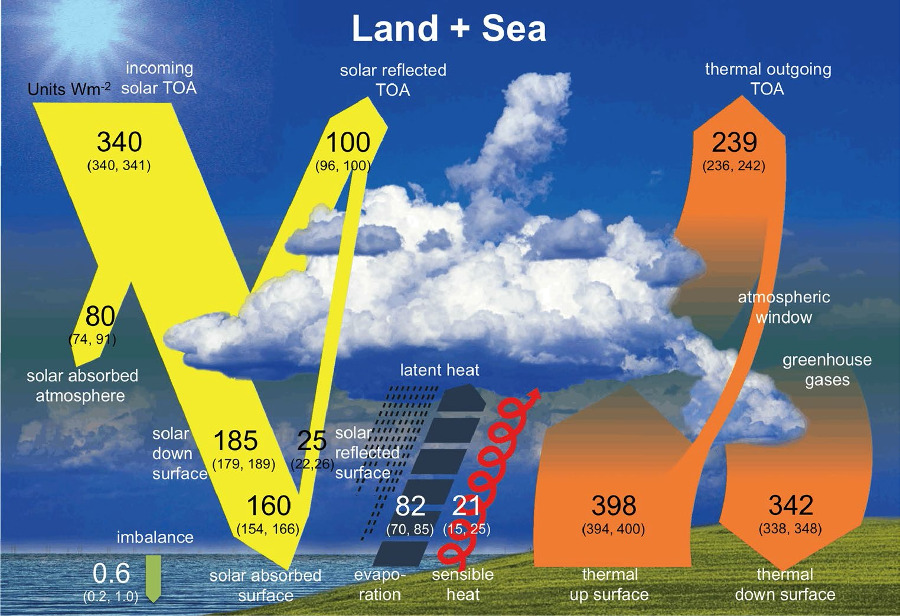
\includegraphics[scale = 0.3]{./Bilder_Klima/Bilanz.jpg}
\caption{\label{fig_Bilanz}%
Einfaches Diagramm zur Veranschaulichung des radiativen Energiehaushalts
der Atmosph\"are. TOA = top of atmosphere. Die Zahlen bezeichnen eine
Strahlungsintensit\"at (in Watt pro Quadratmeter). In Klammern ist jeweils
das Intervall der Unsicherheit angegeben. (Aus \cite{Sanchez})} 
\end{SCfigure}

Im Folgenden verwenden wir auch das Kirchhoff'sche Strahlungsgesetz, wonach der
Absorptionskoeffizient und der Emissionskoeffizient eines K\"orpers gleich sind. Wir setzen
hier die integrierte diffuse Strahlung voraus, d.h.\ wir betrachten keine Richtungsabh\"angigkeiten. 
Allerdings ber\"ucksichtigen einige der Klimamodelle eine Frequenzabh\"angigkeit dieser
Koeffizienten. Die Interpretation sogenannter Emissionskoeffizienten in diesem Kapitel
bedeutet meist, dass die Atmosp\"are f\"ur bestimmte Frequenzen
absorbierend und f\"ur andere Frequenzen durchl\"assig ist. Daher ist die Forderungg, dass
die frequenzabh\"angige Absorbtion gleich der entsprechenden Emission ist, eher eine
N\"aherung. 


\subsection{Klimamodell 1 - ohne Atmosph\"are}

Wir betrachten zun\"achst ein sehr einfaches Klimamodell, bei dem folgende Faktoren
ber\"ucksichtigt werden:
\begin{enumerate}
\item
eine konstante Intensit\"at der Sonnenstrahlung oberhalb der Atmosph\"are, dies ist die Solarkonstante 
$S=1\,361\,{\rm J\cdot s^{-1} \cdot m^{-2}}$,
\item
eine konstante Albedo von $a=0,3$,
\item
eine Erdoberfl\"ache, welche die absorbierte Energie in alle Richtungen als
Schwarzk\"orperstrahlung entsprechend ihrer Oberfl\"achentemperatur $T$ abgibt. 
Hier wird das Stefan-Boltzmann-Gesetz 
\begin{equation}
                L=\sigma T^4
\end{equation}                 
angenommen, d.h., die abgestrahlte Intensit\"at $L$ (Energie pro Zeit und Fl\"ache) ist 
proportional zur 4.\ Potenz der
absoluten Temperatur $T$ der Erdoberfl\"ache.
Die Proportionalit\"atskonstante ist die Stefan-Boltzmann-Konstante
$\sigma = 5,67 \cdot 10^{-8}\,{\rm J \cdot {s}^{-1} \cdot m^{-2} \cdot K^{-4}}$.\hyperref[Anm-2]{(2)}  
\end{enumerate}
Bis auf die Oberfl\"achentemperatur der Erde sind alle Parameter bekannt. F\"ur die
gesamte Intensit\"at der absorbierten Strahlung gilt:
\begin{equation}
          L_{\rm ab} = (1 - a ) S \pi R^2 \, .
\end{equation}
Der Faktor $(1-a)$ beschreibt die Reduktion der eingestrahlten Intensit\"at $S$ aufgrund
der Albedo. $\pi R^2$ (wobei $R$ der Radius der Erde ist) beschreibt die Querschnittsfl\"ache
der Erde, die von der Sonnenstrahlung getroffen wird. Meist argumentiert man, dass dies die
Fl\"ache des Schattens hinter der Erde ist, wo die Sonnenstrahlung fehlt, weil sie auf die
Erde getroffen ist. 

Diese absorbierte Intensit\"at muss im Gleichgewicht gleich der emittierten Intensit\"at
sein (siehe Abb.\ \ref{fig_Klima1}). 
Bei der emittierten Intensit\"at soll es sich in diesem Modell um die Intensit\"at der
Schwarzk\"orperstrahlung der Erde bei ihrer Oberfl\"achentemperatur
$T_{\rm s}$ handeln (siehe Abb.\ \ref{fig_Klima1}, (a)):
\begin{equation}
         L_{\rm em} = \sigma T_{\rm s}^4 \, 4 \pi R^2 \, .
\end{equation}
Hier wird als emittierende Fl\"ache die gesamte Oberfl\"ache der Erde angenommen (daher
der Faktor 4). Setzt man $L_{\rm ab}=L_{\rm em}$ folgt
\begin{equation}
      (1-a) S = 4 \sigma T_{\rm s}^4 \hspace{1cm} \Longrightarrow \hspace{1cm}
          T_{\rm s} = \sqrt[4]{\frac{(1-a) S}{4 \sigma}} = 254,6\,{\rm K} \, .
\end{equation}
Nach diesem einfachen Modell m\"usste die durchschnittliche Erdtemperatur knapp 255\,K oder 
$- 18^\circ$C betragten. Das ist nat\"urlich viel zu kalt. Bei diesen Temperaturen w\"aren die
Ozeane gefroren. Die tats\"achliche Jahresdurchschnittstemperatur der Erde liegt (2017) bei $15^\circ$C
oder 288\,K. 

\begin{figure}[htb]
\begin{tikzpicture}
\draw (0,1) -- (7,1);
\filldraw[fill=gray!20] (0,1) -- (7,1) -- (7,0) -- (0,0) -- (0,1);
\draw (2.0,5) -- (2.0,2) -- (1.7,2) -- (2.5,1) -- (3.3,2) -- (3.0,2) -- (3.0,5);
   \draw (4.0,1.1) -- (4.0,4) -- (3.7,4) -- (4.5,5) -- (5.3,4) -- (5.0,4) -- (5.0,1.1);
\draw [->,snake=snake, segment amplitude = 0.4mm, segment length = 2mm,
               line after snake=1mm] (0,5) -- (1,1.2);
\draw [->,snake=snake, segment amplitude = 0.4mm, segment length = 2mm,
               line after snake=1mm] (0.4,5) -- (1.4,1.2);
\draw [->,snake=snake, segment amplitude = 0.4mm, segment length = 4mm,
               line after snake=1mm] (5.6,1.2) -- (6.6,5);
\draw [->,snake=snake, segment amplitude = 0.4mm, segment length = 4mm,
               line after snake=1mm] (6,1.2) -- (7,5);
\draw (3.5,0.5) node {$T_{\rm S}$};
\draw (3.5,5) node {(a)};
\draw (2,3) node {$L_{\rm ab}=\frac{(1-a)S}{4}$};
\draw (5,3) node {$L_{\rm em}=\sigma T_{\rm s}^4$};
\end{tikzpicture}
\hspace{1cm} %
\begin{tikzpicture}
\draw (0,1) -- (7,1);
\filldraw[fill=gray!20] (0,1) -- (7,1) -- (7,0) -- (0,0) -- (0,1);
\draw (2.0,5) -- (2.0,2) -- (1.7,2) -- (2.5,1) -- (3.3,2) -- (3.0,2) -- (3.0,5);
   \draw (4.0,1.1) -- (4.0,4) -- (3.7,4) -- (4.5,5) -- (5.3,4) -- (5.0,4) -- (5.0,1.1);
\draw [->,snake=snake, segment amplitude = 0.4mm, segment length = 2mm,
               line after snake=1mm] (0,5) -- (1,1.2);
\draw [->,snake=snake, segment amplitude = 0.4mm, segment length = 2mm,
               line after snake=1mm] (0.4,5) -- (1.4,1.2);
\draw [->,snake=snake, segment amplitude = 0.4mm, segment length = 4mm,
               line after snake=1mm] (5.6,1.2) -- (6.6,5);
\draw [->,snake=snake, segment amplitude = 0.4mm, segment length = 4mm,
               line after snake=1mm] (6,1.2) -- (7,5);
\draw (3.5,5) node {(b)};
\draw (3.5,0.5) node {$T_{\rm s}$};
\draw (2,3) node {$L_{\rm ab}=\frac{(1-a)S}{4}$};
\draw (5,3) node {$L_{\rm em}=\hat{\epsilon} \sigma T_{\rm s}^4$};
\end{tikzpicture}
\caption{\label{fig_Klima1}%
Zwei einfache Klimamodelle. (a) In diesem Modell wird s\"amtliche von der Sonne einfallende
Strahlung (abz\"uglich der Albedo) 
von der Erdoberfl\"ache absorbiert und von dieser als Schwarzk\"orperstrahlung wieder
in den Weltraum abgegeben. (b) In diesem Modell gibt die Erdoberfl\"ache ebenfalls alle absorbierte 
Strahlung wieder ab, allerdings nicht als Schwarzk\"orperstrahlung sondern um einen
Faktor $\hat{\epsilon}$ geringer. Dieser Faktor beschreibt den Einfluss des Treibhauseffekts, 
gibt aber keine Erkl\"arung.}
\end{figure}

\subsection{Klimamodell 2 - ohne Atmosph\"arenschicht, mit Emissionsfaktor}

Es gibt mehrere Gr\"unde, weshalb das erste Klimamodell eine deutlich zu tiefe
Oberfl\"achentemperatur der Erde liefern k\"onnte. Zum Einen
k\"onnte es eine Energiequelle geben, die bisher nicht ber\"ucksichtigt wurde. Daf\"ur
kommt praktisch nur die Erde selbst in Frage, insbesondere die Kernzerf\"alle im Inneren
der Erde. Hier zeigt eine genauere \"Uberlegung jedoch, dass dieser Effekt zu klein ist und
f\"ur die Klimabetrachtungen nicht ber\"ucksichtigt zu werden braucht.  

Weiterhin k\"onnte die Annahme falsch sein, dass die Erde eine Schwarzk\"orperstrahlung
zu einer Temperatur $T$ abgibt, die ihrer Oberfl\"achentemperatur entspricht. Wir f\"uhren f\"ur
unser zweites Klimamodell einen Emissionsfaktor $\hat{\epsilon}$ ein, setzen also f\"ur die
emittierte Intensit\"at
\begin{equation}
         L_{\rm em} = \hat{\epsilon} \sigma T^4 \, 4 \pi R^2 
\end{equation}
an. $\hat{\epsilon}=1$ entspricht dem alten Modell. Man spricht in diesem Fall auch schon mal
von einem \glqq grauen Strahler\grqq\ (siehe Abb.\ \ref{fig_Klima1}(b)). Wir erhalten nun f\"ur die
Oberfl\"achentemperatur der Erde:
\begin{equation}
      (1-a) S = 4 \hat{\epsilon} \sigma T^4 \hspace{1cm} \Longrightarrow \hspace{1cm}
          T = \sqrt[4]{\frac{(1-a) S}{4 \hat{\epsilon} \sigma}} = \sqrt[4]{\frac{1}{\hat{\epsilon}}} ~ 254,6\,{\rm K} \, .
\end{equation}
Setzen wir f\"ur $T$ die beobachtete Oberfl\"achentemperatur von 288\,K ein, erhalten
wir $\hat{\epsilon} = 0,61$. Wir haben an dieser Stelle unser \glqq Klimamodell\grqq\ nicht zur
Bestimmung der Oberfl\"achentemperatur $T$ benutzt, sondern zur Bestimmung von
$\hat{\epsilon}$. Gelegentlich wird behauptet, der niedrigere Wert von $\hat{\epsilon}$ beschreibe 
den Treibhauseffekt. Das ist zwar nicht falsch, bedarf aber einer Erkl\"arung. 
Inwieweit $\hat{\epsilon}$ direkt gemessen und somit aus diesem Modell die
Oberfl\"achentemperatur der Erde bestimmt werden kann, werden wir noch
diskutieren. 

\subsection{Klimamodell 3 - eine total absorbierende Atmosph\"arenschicht}

Wir betrachten nun ein Modell, bei dem zwischen der einfallenden Strahlung,
die durch die Solarkonstante gegeben ist, und der ausfallenden Strahlung, die in
den bisherigen beiden Modellen durch die Temperatur der Erdoberfl\"ache
gegeben ist, noch eine Schicht liegt, welche den Einfluss der Treibhausgase
beschreiben soll. Diese Schicht sei vollkommen durchl\"assig f\"ur die einfallende
(kurzwellige) Strahlung der Sonne, sie absorbiere aber die langwellige Strahlung zur Temperatur $T_{\rm s}$,
die von der Erde emittiert wird. Au\ss erdem emittiere sie eine langwellige Strahlung zu ihrer
Atmosph\"arentemperatur $T_{\rm a}$ (siehe Abb.\ \ref{fig_Klima2}). Diese Emission erfolgt
sowohl in Richtung Weltraum (nach oben) als auch zur\"uck in Richtung Erdoberfl\"ache.
Wir haben es nun also mit zwei Temperaturen zu tun: einmal die Temperatur
der Erdoberfl\"ache $T_{\rm s}$ sowie weiterhin die Temperatur $T_{\rm a}$ der Atmosph\"arenschicht,
die wir uns als sehr d\"unn denken. 
 
\begin{SCfigure}[30][htb]
\begin{tikzpicture}
\draw (0,1) -- (9,1);
\filldraw[fill=gray!20] (0,1) -- (9,1) -- (9,0) -- (0,0) -- (0,1);
\filldraw[fill=gray!20] (0,3) -- (2,3) -- (2,2.5) -- (0,2.5) -- (0,3);
\filldraw[fill=gray!20] (3,3) -- (9,3) -- (9,2.5) -- (3,2.5) -- (3,3);
\draw (2.0,5) -- (2.0,2) -- (1.7,2) -- (2.5,1) -- (3.3,2) -- (3.0,2) -- (3.0,5);
\draw (4.5,1.0) -- (4.5,1.5) -- (4.2,1.5) -- (5.0,2.5) -- (5.8,1.5) -- (5.5,1.5) -- (5.5,1.0);
\draw (6.5,2.5) -- (6.5,1.5) -- (6.3,1.5) -- (6.8,1) -- (7.3,1.5) -- (7.1,1.5) -- (7.1,2.5);
\draw (5.7,3.0) -- (5.7,4.5) -- (5.5,4.5) -- (6.0,5) -- (6.5,4.5) -- (6.3,4.5) -- (6.3,3.0);
\draw [->,snake=snake, segment amplitude = 0.4mm, segment length = 2mm,
               line after snake=1mm] (0,5) -- (1,1.1);
\draw [->,snake=snake, segment amplitude = 0.4mm, segment length = 2mm,
               line after snake=1mm] (0.4,5) -- (1.4,1.1);
\draw [->,snake=snake, segment amplitude = 0.4mm, segment length = 4mm,
               line after snake=1mm] (7.6,1.1) -- (8.0,2.6);
\draw [->,snake=snake, segment amplitude = 0.4mm, segment length = 4mm,
               line after snake=1mm] (8,1.1) -- (8.4,2.6);
\draw [->,snake=snake, segment amplitude = 0.4mm, segment length = 4mm,
               line after snake=1mm] (8.3,2.9) -- (8.7,5);
\draw [->,snake=snake, segment amplitude = 0.4mm, segment length = 4mm,
               line after snake=1mm] (8.5,2.6) -- (8.7,1.1);
\draw (4.5,0.5) node {$T_{\rm s}$};
\draw (6.5,0.5) node {Erdboden};
\draw (4.5,2.75) node {$T_{\rm a}$};
\draw (6.5,2.75) node {Atmosph\"are};
\draw (2.0,4) node {$L_{\rm ab}=\frac{(1-a)S}{4}$};
\draw (4.8,1.9) node {$L_{\rm em}=\sigma T_{\rm s}^4$};
\draw (6.8,1.9) node {$L_{\rm a}=\sigma T_{\rm a}^4$};
\draw (6.2,3.9) node {$L_{\rm a}=\sigma T_{\rm a}^4$};
\draw (9.5,0) node {~}; 
\end{tikzpicture}
%\hspace{1cm} %
\caption{\label{fig_Klima2}%
Der Treibhauseffekt - Klimamodell mit einer Atmosph\"arenschicht. Die von der Erdoberfl\"ache
emittierte langwellige Strahlung wird in der Atmosph\"are absorbiert und als
Schwarzk\"orperstrahlung zur Atmosph\"arentemperatur $T_a$ sowohl in
den Weltraum als auch zur\"uck zur Erdoberfl\"ache emittiert.}
\end{SCfigure}

F\"ur beide Schichten - Erdoberfl\"ache und Atmosph\"are - stellen wir nun
Bilanzgleichungen auf. Dabei nehmen wir an, dass die Atmosph\"are nur Energie
von der Erdoberfl\"ache erh\"alt, die entsprechend dem Stefan-Boltzmann-Gesetz
durch $L_{\rm em}=\sigma T_{\rm S}^4$ gegeben ist. Au\ss erdem emittiere die
Atmosph\"are die Energie in zwei Richtungen - nach oben und nach unten - 
entsprechend ihrer Temperatur $T_{\rm a}$. Wir erhalten somit die folgenden zwei
Bilanzgleichungen ((s) f\"ur \glqq surface\grqq, d.h.\ die Bilanzgleichung des Erdbodens,
und (a) f\"ur die Bilanzgleichung der Atmosph\"arenschicht):
\begin{equation}
            (s) \hspace{0.5cm}  \frac{(1-a)}{4} S  +  \sigma T_{\rm a}^4 = \sigma T_{\rm s}^4 \hspace{2cm}
            (a) \hspace{0.5cm}  \sigma T_{\rm s}^4  = 2 \sigma T_{\rm a}^4 \, .
\end{equation}
Bilanzgleichung ($s$) beschreibt die Strahlungsbilanz der Erdoberfl\"ache: Einfallend 
(linke Seite der Gleichung) ist die
kurzwellige Strahlung der Sonne sowie ein Teil, der von der Atmosph\"are nach unten emittiert wird;
ausfallend ist die langwellige Strahlung, welche die Erdoberfl\"ache entsprechend ihrer
Temperatur $T_{\rm s}$ emittiert. Bilanzgleichung ($a$)
beschreibt die Strahlungsbilanz der Atmosph\"arenschicht (die als d\"unn und von konstanter Temperatur
angenommen wird): Einfallend ist die emittierte langwellige Strahlung der Erde, emittiert werden
zwei Anteile (nach unten und nach oben in den Weltraum) entsprechend der Temperatur $T_{\rm a}$.

Aus der zweiten Gleichung folgt unmittelbar $T_{\rm s} = \sqrt[4]{2}\, T_{\rm a}$, die Temperatur der
Erdoberfl\"ache ist also um den Faktor $\sqrt[4]{2} \approx 1,1892$ h\"oher als die Temperatur $T_{\rm a}$ der
Atmosph\"are. Setzt man die zweite Bilanzgleichung in die erste ein, erh\"alt man f\"ur die Atmosph\"arentemperatur
den Wert des ersten Modells $T_{\rm a} \approx 254,6$\,K oder $-18^\circ$C. Dies ist auch plausibel, weil f\"ur das
Gesamtsystem die Strahlungsbilanz ebenfalls ausgeglichen sein soll. F\"ur die Temperatur der Erdoberfl\"ache
erhalten wir nun $T_{\rm s}\approx 303$\,K oder $30^\circ$C. Das ist etwas zu warm wenn man bedenkt, dass die
mittlere Temperatur der Erdoberfl\"ache eher bei $15^\circ$C liegt. 

An diese Modell wird offensichtlich, dass die Temperatur, die man aus einer gro\ss en Entfernung von der
Erde beobachtet, nicht die Temperatur der Erdoberfl\"ache ist (wie in dem ersten Modell), sondern die
Temperatur der (oberen) Atmosph\"arenschicht. 

\subsection{Klimamodell 4 - eine teilabsorbierende Atmosph\"arenschicht}

\begin{SCfigure}[30][htb]
\begin{tikzpicture}
\draw (0,1) -- (9,1);
\filldraw[fill=gray!20] (0,1) -- (9,1) -- (9,0) -- (0,0) -- (0,1);
\filldraw[fill=gray!20] (0,3) -- (2,3) -- (2,2.5) -- (0,2.5) -- (0,3);
\filldraw[fill=gray!20] (3,3) -- (3.7,3) -- (3.7,2.5) -- (3,2.5) -- (3,3);
\filldraw[fill=gray!20] (4.1,3) -- (9,3) -- (9,2.5) -- (4.1,2.5) -- (4.1,3);
\draw (2.0,5) -- (2.0,2) -- (1.7,2) -- (2.5,1) -- (3.3,2) -- (3.0,2) -- (3.0,5);
\draw (4.7,1.0) -- (4.7,1.5) -- (4.4,1.5) -- (5.1,2.5) -- (5.8,1.5) -- (5.5,1.5) -- (5.5,1.0);
\draw (3.7,1.0) -- (3.7,4) -- (3.5,4) -- (3.9,5) -- (4.3,4) -- (4.1,4) -- (4.1,1.0);
\draw (6.5,2.5) -- (6.5,1.5) -- (6.3,1.5) -- (6.8,1) -- (7.3,1.5) -- (7.1,1.5) -- (7.1,2.5);
\draw (5.7,3.0) -- (5.7,4.5) -- (5.5,4.5) -- (6.0,5) -- (6.5,4.5) -- (6.3,4.5) -- (6.3,3.0);
\draw [->,snake=snake, segment amplitude = 0.4mm, segment length = 2mm,
               line after snake=1mm] (0,5) -- (1,1.1);
\draw [->,snake=snake, segment amplitude = 0.4mm, segment length = 2mm,
               line after snake=1mm] (0.4,5) -- (1.4,1.1);
\draw [->,snake=snake, segment amplitude = 0.4mm, segment length = 4mm,
               line after snake=1mm] (7.6,1.1) -- (8.6,5.0);
\draw [->,snake=snake, segment amplitude = 0.4mm, segment length = 4mm,
               line after snake=1mm] (7.8,1.1) -- (8.2,2.6);
\draw [->,snake=snake, segment amplitude = 0.4mm, segment length = 4mm,
               line after snake=1mm] (8,1.1) -- (8.4,2.6);
\draw [->,snake=snake, segment amplitude = 0.4mm, segment length = 4mm,
               line after snake=1mm] (8.3,2.9) -- (8.8,5);
\draw [->,snake=snake, segment amplitude = 0.4mm, segment length = 4mm,
               line after snake=1mm] (8.5,2.6) -- (8.7,1.1);
\draw (4.5,0.5) node {$T_{\rm s}$};
\draw (6.5,0.5) node {Erdboden};
\draw (5.0,2.75) node {$T_{\rm a}$};
\draw (6.5,2.75) node {Atmosph\"are};
\draw (2.0,4) node {$L_{\rm ab}=\frac{(1-a)S}{4}$};
\draw (4.3,3.8) node {$L_{\rm em}=$};
\draw (4.1,3.4) node {$(1-\epsilon) \sigma T_{\rm s}^4$};
\draw (5.1,1.9) node {$L_{\rm em}=\epsilon \sigma T_{\rm s}^4$};
\draw (7.0,1.9) node {$L_{\rm a}=\epsilon \sigma T_{\rm a}^4$};
\draw (6.5,4.2) node {$L_{\rm a}=\epsilon \sigma T_{\rm a}^4$};
\draw (9.5,0) node {~}; 
\end{tikzpicture}
%\hspace{1cm} %
\caption{\label{fig_Klima3}%
Effektiver Treibhauseffekt mit einer teilweise absorbierenden
Atmosph\"arenschicht. Die von der Erdoberfl\"ache
emittierte langwellige Strahlung wird teilweise in der Atmosph\"are absorbiert 
und teilweise durchgelassen. Der absorbierte Anteil wird als \glqq graue Strahlung\grqq\
mit Emissionskoeffizienten $\epsilon$ zur Atmosph\"arentemperatur $T_a$ sowohl in
den Weltraum als auch zur\"uck zur Erdoberfl\"ache emittiert.}
\end{SCfigure}

In diesem Klimamodell wird angenommen, dass die Atmosph\"arenschicht nur einen Teil
der von der Erde emittierten langwelligen Strahlung absorbiert (parametrisiert durch den Parameter $\epsilon$)
und einen Teil direkt durchl\"asst (siehe Abb.\ \ref{fig_Klima3}). Entsprechend den
Kirchhoff'schen Strahlungsgesetzen, wonach Absorptions- und Emissionskoeffizient eines
K\"orpers f\"ur eine gegebene Wellenl\"ange gleich sind (Richtungsabh\"angigkeiten werden hier
vernachl\"assigt), wird bei
diesem Modell angenommen, dass die Atmosph\"are f\"ur bestimmte Wellenl\"angen
transparent ist - und entsprechend bei diesen Wellenl\"angen auch nicht emittiert - 
und andere Wellenl\"angen absorbiert, die dann auch wieder (diffus, also in alle Richtungen) emittiert werden. 

Nun lauten die Bilanzgleichungen:
\begin{equation}
            (s) \hspace{0.5cm}  \frac{(1-a)}{4} S  + \epsilon \sigma T_{\rm a}^4 
                = ((1-\epsilon) + \epsilon) \sigma T_{\rm s}^4 = \sigma T_{\rm s}^4 \hspace{1.8cm}
            (a) \hspace{0.5cm}  \epsilon \sigma T_{\rm s}^4  = 2 \epsilon \sigma T_{\rm a}^4 \, .
\end{equation}
Aus der zweiten Gleichung (f\"ur die Atmosph\"arenschicht) folgt:
\begin{equation}
                 T^4_{\rm s} = 2 \, T^4_{\rm a}  \hspace{1cm} {\rm bzw.} \hspace{1cm}  
                 T_{\rm s} = \sqrt[4]{2} ~ T_{\rm a}  \, .  
\end{equation}
Wenn wir dies in die erste Gleichung einsetzen, erhalten wir f\"ur die Atmosph\"arentemperatur:
\begin{equation}
           T_{\rm a} = \sqrt[4]{\frac{(1-a)S}{4} \frac{1}{2-\epsilon}}
                                =  \sqrt[4]{\frac{1}{2-\epsilon}} ~ 254,6\,{\rm K} 
\end{equation}
und damit f\"ur die Bodentemperatur der Erde:
\begin{equation}
           T_{\rm s} = \sqrt[4]{\frac{(1-a)S}{4} \frac{2}{2-\epsilon}}
                                =  \sqrt[4]{\frac{2}{2-\epsilon}}  ~  254,6\,{\rm K} \, .
\end{equation}
F\"ur $\epsilon \rightarrow 0$ erhalten wir unser erstes Modell wieder: Die Atmosph\"are
emittiert keine Strahlung mehr (ihre Temperatur w\"are $T_{\rm a} = (1/\sqrt[4]{2})\cdot 254,6$\,K
$\approx 214,1$\,K, bei der aber praktisch keine Strahlung emittiert wird). S\"amtliche von der Erdoberfl\"ache
absorbierte Energie wird als Schwarzk\"orperstrahlung bei $254,6$\,K wieder in den Weltraum 
abgestrahlt. F\"ur $\epsilon \rightarrow 1$ erhalten wir das vorherige Modell: Die Atmosph\"arentemperatur
betr\"agt $254,6$\,K und die Temperatur der Erdoberfl\"ache ist $T_{\rm s}=\sqrt[4]{2}\cdot 254,6\,{\rm K}
\approx 303$\,K. 

Wenn wir nun umgekehrt f\"ur die durchschnittliche Oberfl\"achentemperatur der Erde den Wert $288$\,K
annehmen, erhalten wir den Wert $\epsilon \approx 0,7785$, und f\"ur die Atmosph\"arentemperatur
folgt daraus ein Wert von rund $242$\,K. \"Uber Polareis (siehe Abb.\ \ref{fig_updown}) w\"urde sich f\"ur
eine Erdtemperatur von $268$\,K eine Atmosph\"arentemperatur von $226$\,K ergeben, was recht gut
mit den beobachteten Werten \"ubereinstimmt. Der Vorteil dieses Modells
ist, dass wir hier einige Effekte studieren und interpretieren k\"onnen, die bisher nicht so
offensichtlich waren.

\begin{SCfigure}[30][htb]
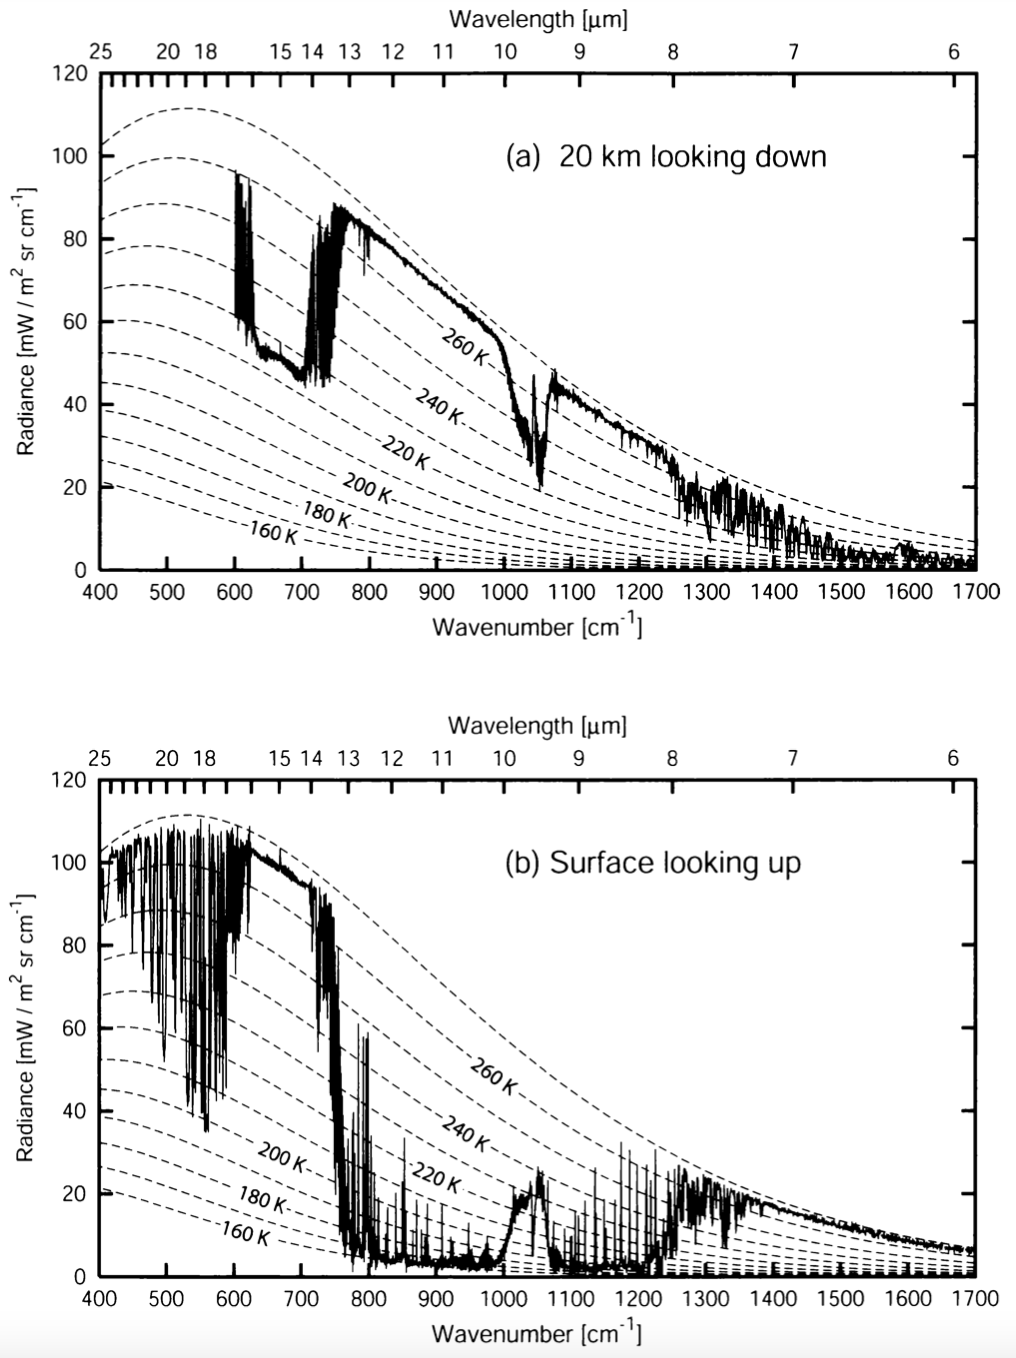
\includegraphics[scale = 0.4]{./Bilder_Klima/Petty.png}
\caption{\label{fig_updown}%
(oben) Spektralzerlegung der Erdstrahlung aus gro\ss er H\"ohe betrachtet.
(unten) Spektrale Zerlegung der Atmosph\"arenstrahlung vom Erdboden aus
betrachtet. Die Diagramme wurden \"uber Polareis aufgenommen. 
Die wellenl\"angenabh\"angigen Kurven werden verglichen mit
Schwarzk\"orperstrahlungen zu verschiedenen Temperaturen. Aus gro\ss er H\"ohe
sieht man Bereiche mit einer Temperatur von rund 268\,K - diese entsprechen
der Erdoberfl\"ache - und andere Bereiche mit einer Temperatur von rund 226\,K - 
diese entsprechen der oberen Atmosph\"are. In Wellenl\"angenbereichen, in denen
die Atmosph\"are lichtdurchl\"assig ist, sieht man im oberen Bild eine Temperatur von rund
268\,K, also den Erdboden, und im unteren Bild eine sehr niedrige Temperatur entsprechend
dem Weltraum. Aus \cite{Petty}.}  
\end{SCfigure}

\begin{enumerate}
\item
F\"ur $\epsilon \neq 1$ oder 0 entspricht die Strahlung, welche die Erde in den Weltraum
abgibt - die also von einer gro\ss en H\"ohe aus beobachtet wird - nicht einer
Schwarzk\"orperstrahlung zu einer festen Temperatur sondern einer Strahlung zu zwei
Temperaturen. Damit erh\"alt der Parameter $\hat{\epsilon}$ aus dem zweiten Modell eine
anschauliche Bedeutung: Bei manchen
Wellenl\"angen ist die Atmosph\"are durchl\"assig und man sieht somit bei diesen Wellenl\"angen aus 
gro\ss er H\"ohe die Oberfl\"ache der Erde (und ihre Temperatur). Bei anderen
Wellenl\"angen ist die Atmosph\"are absorbierend und undurchsichtig. Bei diesen Wellenl\"angen
sieht man aus einer gro\ss en H\"ohe nur die obere Atmosph\"arenschicht und dies bei einer
deutlich niedrigeren Temperatur (vgl.\ Abb.\ \ref{fig_updown}).
\item
Wenn $\epsilon$ gr\"o\ss er wird, also mehr Strahlung von der Atmosph\"are absorbiert wird,
nimmt die Temperatur der Erdoberfl\"ache zu. Dies ist der eigentliche Treibhauseffekt. 
Gleichzeitig nimmt in diesem Modell aber auch die Temperatur der oberen Atmosph\"arenschicht, von der
aus die Strahlung in den Weltraum abgegeben wird, zu. Sie ist allerdings insgesamt k\"alter
als in dem Klimamodell 3. Da die einfallende Intensit\"at
(die Solarkonstante und die Albedo) mehr oder weniger konstant bleibt, muss auch die
abgegebene Intensit\"at in der Summe konstant bleiben. Wenn aber von der Erdoberfl\"ache
Strahlung zu einer h\"oheren Temperatur in den Weltraum abgegeben wird, muss die Strahlung
von den oberen Atmosph\"arenschichten zu einer tieferen Temperatur geh\"oren.
\end{enumerate} 

\subsection{Ein einfaches Klimamodell f\"ur die Venus}

Die Atmosph\"are der Venus enth\"alt rund 96\% Kohlendioxid. Der Abstand Venus-Sonne
betr\"agt ungef\"ahr $0,72$\,AU (astronomische Einheiten) und somit ist die Solarkonstante
an der Oberfl\"ache der Venusatmosph\"are um rund das Inverse von $(0,72)^2 \approx 0,52$,
also knapp das Doppelte, gr\"o\ss er als 
auf der Erde (dies beruht auf dem $1/r^2$-Gesetz der Intensit\"at einer Strahlung als Funktion des
Abstands von der Strahlungsquelle). Allerdings ist die Albedo der Venus mit rund $0,75$ deutlich gr\"o\ss er als die
der Erde (von au\ss en erscheint die Venus vollkommen wolkenbedeckt). 
Insgesamt m\"usste es daher auf der Venus k\"alter sein, als auf der Erde. 
Doch die Oberfl\"achentemperatur der Venus betr\"agt \"uber $460^\circ$C. Um zu sehen, wie
eine dickere absorbierende Atmosph\"arenschicht die Oberfl\"achentemperatur beeinflusst,
betrachten wir folgendes Atmosph\"arenmodell (siehe Abb.\ \ref{fig_Klima4}). 

\begin{SCfigure}[30][htb]
\begin{tikzpicture}
%\draw (0,1) -- (9,1);
\filldraw[fill=gray!20] (0,1) -- (9,1) -- (9,0) -- (0,0) -- (0,1);
\filldraw[fill=gray!20] (0,3) -- (2,3) -- (2,2.5) -- (0,2.5) -- (0,3);
\filldraw[fill=gray!20] (3,3) -- (9,3) -- (9,2.5) -- (3,2.5) -- (3,3);
\filldraw[fill=gray!20] (0,5) -- (2,5) -- (2,4.5) -- (0,4.5) -- (0,5);
\filldraw[fill=gray!20] (3,5) -- (9,5) -- (9,4.5) -- (3,4.5) -- (3,5);
\draw (2.0,6) -- (2.0,2) -- (1.7,2) -- (2.5,1) -- (3.3,2) -- (3.0,2) -- (3.0,6);
\draw (4.5,1.0) -- (4.5,1.5) -- (4.2,1.5) -- (5.0,2.5) -- (5.8,1.5) -- (5.5,1.5) -- (5.5,1.0);
\draw (6.5,2.5) -- (6.5,1.5) -- (6.3,1.5) -- (6.8,1) -- (7.3,1.5) -- (7.1,1.5) -- (7.1,2.5);
\draw (4.8,3.0) -- (4.8,4.0) -- (4.6,4.0) -- (5.1,4.5) -- (5.6,4.0) -- (5.4,4.0) -- (5.4,3.0);
\draw (6.5,4.5) -- (6.5,3.5) -- (6.3,3.5) -- (6.7,3) -- (7.1,3.5) -- (6.9,3.5) -- (6.9,4.5);
\draw (5.8,5.0) -- (5.8,5.7) -- (5.6,5.7) -- (6,6.2) -- (6.4,5.7) -- (6.2,5.7) -- (6.2,5.0);
\draw [->,snake=snake, segment amplitude = 0.4mm, segment length = 2mm,
               line after snake=1mm] (0,6) -- (1,1.1);
\draw [->,snake=snake, segment amplitude = 0.4mm, segment length = 2mm,
               line after snake=1mm] (0.4,6) -- (1.4,1.1);
\draw [->,snake=snake, segment amplitude = 0.4mm, segment length = 4mm,
               line after snake=1mm] (7.6,1.1) -- (8.0,2.6);
\draw [->,snake=snake, segment amplitude = 0.4mm, segment length = 4mm,
               line after snake=1mm] (7.8,1.1) -- (8.2,2.6);
\draw [->,snake=snake, segment amplitude = 0.4mm, segment length = 4mm,
               line after snake=1mm] (8,1.1) -- (8.4,2.6);
\draw [->,snake=snake, segment amplitude = 0.4mm, segment length = 4mm,
               line after snake=1mm] (8.5,2.6) -- (8.7,1.0);
\draw [->,snake=snake, segment amplitude = 0.4mm, segment length = 4mm,
               line after snake=1mm] (7.9,2.9) -- (8.2,4.6);
\draw [->,snake=snake, segment amplitude = 0.4mm, segment length = 4mm,
               line after snake=1mm] (8.1,2.9) -- (8.4,4.6);
\draw [->,snake=snake, segment amplitude = 0.4mm, segment length = 4mm,
               line after snake=1mm] (8.5,4.6) -- (8.7,2.9);
\draw [->,snake=snake, segment amplitude = 0.4mm, segment length = 4mm,
               line after snake=1mm] (8.2,4.9) -- (8.4,6.2); 
\draw (4.5,0.5) node {$T_{\rm s}$};
\draw (6.5,0.5) node {Oberfl\"ache Venus};
\draw (4.5,2.75) node {$T_{\rm a1}$};
\draw (6.5,2.75) node {Atmosph\"are 1}; 
\draw (4.5,4.75) node {$T_{\rm a2}$};
\draw (6.5,4.75) node {Atmosph\"are 2};
\draw (2.0,4) node {$L_{\rm ab}=\frac{(1-a)S}{4}$};
\draw (4.8,1.9) node {$L_{\rm em}=\sigma T_{\rm s}^4$};
\draw (6.8,1.9) node {$L_{\rm a1}=\sigma T_{\rm a1}^4$};
\draw (5.0,3.7) node {$L_{\rm a1}=\sigma T_{\rm a1}^4$};
\draw (6.8,3.7) node {$L_{\rm a2}=\sigma T_{\rm a2}^4$};
\draw (6.0,5.4) node {$L_{\rm a2}=\sigma T_{\rm a2}^4$};
\draw (9.2,0) node {~}; 
\end{tikzpicture}
%\hspace{1cm} %
\caption{\label{fig_Klima4}%
Modell f\"ur den Treibhauseffekt der Venus - ein Klimamodell mit zwei Atmosph\"arenschichten. 
Die von der Venusoberfl\"ache
emittierte langwellige Strahlung wird in der ersten Atmosph\"are absorbiert und als
Schwarzk\"orperstrahlung zur Atmosph\"arentemperatur $T_{\rm a1}$ zur zweiten Schicht wie
auch zur\"uck zur Venusoberfl\"ache emittiert. Die zweite Schicht mit der Temperatur
$T_{\rm a2}$ emittiert Strahlung zur\"uck zur ersten Schicht und in den Weltraum.}
\end{SCfigure}

Die Bilanzgleichungen sind nun (wobei durch die Stefan-Boltzmann-Konstante $\sigma$ dividiert
wurde):
\begin{equation}
       (g) \hspace{0.5cm}   \frac{(1-a)S}{4\sigma} + T_{\rm a1}^4 = T_{\rm s}^4 
       \hspace{1cm} (a1) \hspace{0.5cm}   
        T_{\rm s}^4 + T_{\rm a2}^4 = 2  T_{\rm a1}^4 
       \hspace{1cm} (a2) \hspace{0.5cm}   
        T_{\rm a1}^4 = 2  T_{\rm a2}^4  \, 
\end{equation}
Aus diesen Gleichungen erhalten wir (die Zahlenwerte gelten zum besseren Vergleich mit den
vorherigen Modellen f\"ur die Albedo und die Solarkonstante der Erde):
\begin{eqnarray}
         T_{\rm a2} &=& \sqrt[4]{\frac{(1-a) S}{4 \sigma}} = 254,6\,{\rm K}  \\
         T_{\rm a1} &=& \sqrt[4]{2} T_{\rm a2} =  \sqrt[4]{2}\cdot
                                   \sqrt[4]{\frac{(1-a) S}{4 \sigma}} = \sqrt[4]{2}\cdot 254,6\,{\rm K} 
                                      \approx 302,8\, {\rm K} \\
         T_{\rm s} &=& \sqrt[4]{3} T_{\rm a2} 
                                =  \sqrt[4]{3} \cdot \sqrt[4]{\frac{(1-a) S}{4 \sigma}} = \sqrt[4]{3} \cdot 254,6\,{\rm K} 
                                      \approx 335,1\, {\rm K} 
\end{eqnarray}
Die oberste Atmosph\"arenschicht beh\"alt somit ihre Temperatur von $254,6$\,K, wohingegen die
Temperatur am Boden im Vergleich zu dem Einschicht-Modell nochmals gewachsen ist. Man kann
sich nun leicht \"uberlegen, dass sich dieses Verhalten bei mehreren Atmosph\"arenschichten fortsetzt. 
Letztendlich erh\"alt man, dass immer dieselbe Temperatur von $254,6$\,K in den Weltraum abgestrahlt
wird, diese Temperatur zu den tieferen Schichten hin zunimmt und am Boden theoretisch einen
beliebig hohen Wert annehmen kann. Auch wenn sich die Zahlenwerte hier auf die Albedo und die
Solarkonstante der Erde beziehen, kann man das Modell leicht auf Venus \"ubertragen. Durch die hohe
Konzentration an ${\rm CO}_2$ (sowie die Tatsache, dass die Atmosph\"are der Venus fast 90 mal
dichter ist als die der Erde)
wirken dort effektiv viele Atmosph\"arenschichten total absorbierend.

Modelle f\"ur die Atmosph\"aren anderer Planeten oder auch von Monden anderer Planeten (z.B.\ der
Jupiter- und Saturnmonde) sind auch f\"ur die Klimaphysik von Interesse, weil man an diesen
Modellen testen kann, ob die Zusammenh\"ange durch die einfachen Modelle schon nahezu korrekt
wiedergegeben werden und somit diese einfachen Modelle der Realit\"at entsprechen.

\subsection{Klimamodell 5 - Erw\"armung der Troposph\"are und Abk\"uhlung der Stratosph\"are}
\label{sec_Klima5}

Nun betrachten wir ein Klimamodell mit zwei Atmosph\"arenschichten, von denen
eine Schicht n\"aherungsweise die Verh\"altnisse in der Troposph\"are und eine zweite
Schicht die Verh\"altnisse in der Stratosph\"are beschreibt. Es ist das allgemeinste Modell in diesem
Kapitel und man erh\"alt alle vorherigen Modelle f\"ur spezielle Werte der Parameter. 

Die Stratosph\"are
zeichnet sich dadurch aus, dass sie einen Teil der einfallenden Sonnenstrahlung
absorbiert (insbesondere im UV-Bereich durch das in der Stratosph\"are vorhandene
Ozon) und in W\"arme umwandelt. Ansonsten wirken sowohl die Troposph\"are als
auch die Stratosph\"are als \glqq graue Strahler\grqq, die bestimmte Wellenl\"angen
absorbieren und emittieren und andere Wellenl\"angen transmittieren und in diesem
Bereich auch nicht emittieren (siehe Abb.\ \ref{fig_Klima5}). Die zugeh\"origen
Emissionsfaktoren (gleich Absorptionsfaktoren) $\epsilon_{\rm tro}$ und $\epsilon_{\rm str}$
geben wieder den Anteil einer Strahlung an, die von dieser Schicht absorbiert und
emittiert wird. 

\begin{figure}[htb]
\begin{tikzpicture}
%\draw (0,1) -- (9,1);
\filldraw[fill=gray!20] (0,1) -- (15,1) -- (15,0) -- (0,0) -- (0,1);         %  Erde
\filldraw[fill=gray!20] (0,3) -- (1.7,3) -- (1.7,2.5) -- (0,2.5) -- (0,3);    %    Trop 1
\filldraw[fill=gray!20] (2.7,3) -- (4.9,3) -- (4.9,2.5) -- (2.7,2.5) -- (2.7,3);   %  Trop  2
\filldraw[fill=gray!20] (5.9,3) -- (11.0,3) -- (11.0,2.5) -- (5.9,2.5) -- (5.9,3);   %  Trop  3
\filldraw[fill=gray!20] (11.4,3) -- (15,3) -- (15,2.5) -- (11.4,2.5) -- (11.4,3);  % Trop  4
\filldraw[fill=gray!20] (0,5) -- (1.7,5) -- (1.7,4.5) -- (0,4.5) -- (0,5);        %  Stra 1
\filldraw[fill=gray!20] (2.7,5) -- (5.5,5) -- (5.5,4.5) -- (2.7,4.5) -- (2.7,5);  %  Stra  2
\filldraw[fill=gray!20] (5.9,5) -- (8.6,5) -- (8.6,4.5) -- (5.9,4.5) -- (5.9,5);     %  Stra 3
\filldraw[fill=gray!20] (9.0,5) -- (15,5) -- (15,4.5) -- (9.0,4.5) -- (9.0,5);     %  Stra 4
\draw (1.7,6.5) -- (1.7,2) -- (1.4,2) -- (2.2,1) -- (3.0,2) -- (2.7,2) -- (2.7,5.8);    %  top -> s
\draw (2.7,5.3) -- (2.5,5.3) -- (3.0,5.0) -- (3.5,5.3) -- (3.3,5.3) -- (3.3,6.5);       %  top -> str
%
\draw (4.9,1) -- (4.9,4) -- (4.7,4) -- (5.2,4.5) -- (5.7,4) -- (5.5,4) -- (5.5,3.0);                    %  s  ->  str
\draw (5.5,3.0) -- (5.5,6) -- (5.3,6) -- (5.7,6.5) -- (6.1,6) -- (5.9,6) -- (5.9,1.5);                    %  s  ->  top
\draw (5.9,1.5) -- (5.9,2.0) -- (5.7,2.0) -- (6.2,2.5) -- (6.7,2.0) -- (6.5,2.0) -- (6.5,1.0);  %  s -> tro
%
\draw (8.0,3.0) -- (8.0,4.0) -- (7.8,4.0) -- (8.3,4.5) -- (8.8,4.0) -- (8.6,4.0) -- (8.6,3.6);  %  tro -> str
\draw (8.6,3.6) -- (8.6,6.0) -- (8.4,6.0) -- (8.8,6.5) -- (9.2,6.0) -- (9.0,6.0) -- (9.0,3.0);  %  tro -> top
\draw (8.0,2.5) -- (8.0,1.5) -- (7.8,1.5) -- (8.5,1) -- (9.2,1.5) -- (9,1.5) -- (9,2.5);    %  tro ->  s
%
\draw (11.0,4.5) -- (11.0,1.5) -- (10.8,1.5) -- (11.2,1) -- (11.6,1.5) -- (11.4,1.5) -- (11.4,3.8);    %  str  ->  s
\draw (11.4,3.8) -- (11.4,3.5) -- (11.2,3.5) -- (11.6,3) -- (12.0,3.5) -- (11.8,3.5) -- (11.8,4.5);    %  str  ->  tro
\draw (11.0,5.0) -- (11.0,6) -- (10.8,6) -- (11.4,6.5) -- (12.0,6) -- (11.8,6) -- (11.8,5.0);   %  str ->  top
\draw [->,snake=snake, segment amplitude = 0.4mm, segment length = 2mm,
               line after snake=1mm] (0,6) -- (1,1.1);
\draw [->,snake=snake, segment amplitude = 0.4mm, segment length = 2mm,
               line after snake=1mm] (0.4,6) -- (1.4,1.1);
\draw [->,snake=snake, segment amplitude = 0.4mm, segment length = 2mm,
               line after snake=1mm] (0.8,6) -- (1.1,4.8);
%\draw [->,snake=snake, segment amplitude = 0.4mm, segment length = 4mm,
%               line after snake=1mm] (13.6,1.1) -- (14.0,2.6);
%\draw [->,snake=snake, segment amplitude = 0.4mm, segment length = 4mm,
%               line after snake=1mm] (13.8,1.1) -- (14.2,2.6);
%\draw [->,snake=snake, segment amplitude = 0.4mm, segment length = 4mm,
%               line after snake=1mm] (14,1.1) -- (14.4,2.6);
%\draw [->,snake=snake, segment amplitude = 0.4mm, segment length = 4mm,
%               line after snake=1mm] (14.5,2.6) -- (14.7,1.0);
%\draw [->,snake=snake, segment amplitude = 0.4mm, segment length = 4mm,
%               line after snake=1mm] (13.9,2.9) -- (14.2,4.6);
%\draw [->,snake=snake, segment amplitude = 0.4mm, segment length = 4mm,
%               line after snake=1mm] (14.1,2.9) -- (14.4,4.6);
%\draw [->,snake=snake, segment amplitude = 0.4mm, segment length = 4mm,
%               line after snake=1mm] (14.5,4.6) -- (14.7,2.9);
%\draw [->,snake=snake, segment amplitude = 0.4mm, segment length = 4mm,
%               line after snake=1mm] (14.2,4.9) -- (14.4,6.2); 
\draw (6.8,0.5) node {$T_{\rm s}$};
\draw (8.5,0.5) node {Oberfl\"ache Erde};
\draw (6.6,2.75) node {$T_{\rm tro}$};
\draw (8.1,2.75) node {Troposph\"are}; 
\draw (11.0,4.75) node {$T_{\rm str}$};
\draw (12.5,4.75) node {Stratosph\"are};
\draw (2.1,6.2) node {$L_{\rm sol}=\frac{(1-a)S}{4}$};
\draw (2.2,1.8) node {${\scriptstyle (1-\beta_{\rm str})}$};
\draw (3.0,5.3) node {${\scriptstyle \beta_{\rm str}}$};
\draw (5.7,1.25) node {$L_{\rm s}=\sigma T_{\rm s}^4$};
\draw (6.2,2.2) node {${\scriptstyle \epsilon_{\rm tro}}$};
\draw (5.4,2.7) node {${\scriptstyle (1-\epsilon_{\rm tro})}$};
\draw (5.2,4.1) node {${\scriptstyle \epsilon_{\rm str}}$};
\draw (6.0,5.2) node {${\scriptstyle (1-\epsilon_{\rm str})}$};
\draw (8.5,2.2) node {$L_{\rm tro}=\epsilon_{\rm tro} \sigma T_{\rm tro}^4$};
\draw (8.5,3.3) node {$L_{\rm tro}=\epsilon_{\rm tro} \sigma T_{\rm tro}^4$};
\draw (8.3,4.1) node {${\scriptstyle \epsilon_{\rm str}}$};
\draw (8.8,5.2) node {${\scriptstyle (1-\epsilon_{\rm str})}$};
\draw (11.3,4.2) node {$L_{\rm str}=\epsilon_{\rm str} \sigma T_{\rm str}^4$};
\draw (11.3,5.4) node {$L_{\rm str}=\epsilon_{\rm str} \sigma T_{\rm str}^4$};
\draw (11.65,3.35) node {${\scriptstyle \epsilon_{\rm tro}}$};
\draw (11.5,2.7) node {${\scriptstyle (1-\epsilon_{\rm tro})}$};
\draw (9.2,0) node {~}; 
\end{tikzpicture}
%\hspace{1cm} %
\caption{\label{fig_Klima5}%
Modell f\"ur die Strahlungsbilanz mit einer Troposph\"are und eine Stratosph\"are. Die Stratosph\"are
absorbiert einen Teil der einfallenden Sonnenstrahlung (Absorptionskoeffizient $\beta_{\rm str}$)
und wird dadurch erw\"armt. Au\ss erdem 
absorbiert sie Teile der langwelligen Infrarotstrahlung von der Erdoberfl\"ache und der Troposph\"are.
Die Erdoberfl\"ache absorbiert und emittiert als schwarzer K\"orper und hat somit einen
Emissionskoeffizienten von 1. Die Troposph\"are und Stratosph\"are absorbieren und emittieren als
\glqq graue Strahler\grqq. Die Troposph\"are hat einen Absorptions- und Emissionskoeffizienten
von $\epsilon_{\rm tro}$ und die Stratosph\"are einen entsprechenden Koeffizienten $\epsilon_{\rm str}$.
Der durchgelassene Strahlungsanteil ist jeweils proportional zu $(1-\epsilon_{\rm tro/str})$.
}
\end{figure}

Die Bilanzgleichungen f\"ur die drei Schichten lassen sich anhand von Abb.\ \ref{fig_Klima4} ablesen
und lauten:
\begin{eqnarray}
   \mbox{Erdboden} \hspace{1cm} & &  \hspace{-0.8cm}
      (1-\beta_{\rm str}) \frac{(1-a)S}{4} + \epsilon_{\rm tro} \sigma T_{\rm tro}^4 +
        \epsilon_{\rm str} (1-\epsilon_{\rm tro}) \sigma T_{\rm str}^4 =  \sigma T_{\rm s}^4  \\
 \label{eq_Trop}       
   \mbox{Troposph\"are} \hspace{1cm} & &  \hspace{3.5cm}
       \epsilon_{\rm tro} \sigma T_{\rm s}^4 +
        \epsilon_{\rm str} \epsilon_{\rm tro} \sigma T_{\rm str}^4 = 2 \epsilon_{\rm tro} \sigma T_{\rm tro}^4  \\
   \mbox{Stratosph\"are} \hspace{1cm} & & \hspace{-0.3cm}
        \beta_{\rm str} \frac{(1-a)S}{4} + \epsilon_{\rm tro} \epsilon_{\rm str} \sigma T_{\rm tro}^4 +
        \epsilon_{\rm str} (1-\epsilon_{\rm tro}) \sigma T_{\rm s}^4 =  2 \epsilon_{\rm str} \sigma T_{\rm str}^4 
\end{eqnarray}
Wir k\"onnen diese drei Gleichungen in Matrixform schreiben:
\begin{equation}
    \left( \begin{array}{ccc}  1 &  -\epsilon_{\rm tro} & - \epsilon_{\rm str} (1-\epsilon_{\rm tro}) \\
      - \epsilon_{\rm tro} &  2\epsilon_{\rm tro} &  - \epsilon_{\rm tro} \epsilon_{\rm str} \\ 
     - \epsilon_{\rm str} (1 - \epsilon_{\rm tro}) & - \epsilon_{\rm tro} \epsilon_{\rm str} & 2 \epsilon_{\rm str}
     \end{array} \right) \left( \begin{array}{c}  \sigma T_{\rm s}^4 \\ \sigma T_{\rm tro}^4 \\
       \sigma T_{\rm str}^4 \end{array} \right) 
      =  \left( \begin{array}{c} (1-\beta_{\rm str}) \frac{(1-a)S}{4} \\ 0 \\
             \beta_{\rm str} \frac{(1-a)S}{4}  \end{array} \right) 
\end{equation}
Bildet man die Summe dieser drei Gleichungen erh\"alt man die Bilanz des Gesamtsystems:
\begin{equation}
   \frac{(1-a)S}{4} = (1-\epsilon_{\rm tro})(1- \epsilon_{\rm str}) \sigma T_{\rm s}^4 +
     \epsilon_{\rm tro} (1 - \epsilon_{\rm str}) \sigma T_{\rm tro}^4 +\epsilon_{\rm str} \sigma T_{\rm str}^4 \, .
\end{equation}
In Anhang \ref{Anm_Strat} wird dieses Gleichungssystem gel\"ost. Aus den Gleichungen 
\ref{eq_Tstr}--\ref{eq_Ttro} ergibt sich:
\begin{eqnarray}
\label{eq_Tstr2}
    T_{\rm str}  &=&   \sqrt[4]{ \frac{1}{(2-\epsilon_{\rm str})} 
   \left( 1 + \frac{(1-\epsilon_{\rm str})}{\epsilon_{\rm str}} \beta_{\rm str} \right)}  
           \cdot   254,6\,{\rm K}          \, ,  \\        
    T_{\rm tro}  &=&   \sqrt[4]{   
   \frac{   \big( 2+ \epsilon_{\rm str}(1-\epsilon_{\rm tro})  -  ( \epsilon_{\rm str}+ 
          \epsilon_{\rm tro} (1-\epsilon_{\rm str})) \beta_{\rm str} \big)  }{(2-\epsilon_{\rm str})(2-\epsilon_{\rm tro})}} 
          \cdot    254,6\,{\rm K}          \, ,  \\        
    T_{\rm s}  &=&     \sqrt[4]{
   \frac{\big( (4-\epsilon_{\rm str} \epsilon_{\rm tro})
    -  (2+ \epsilon_{\rm tro} (1-\epsilon_{\rm str})) \beta_{\rm str} \big)}{(2-\epsilon_{\rm str})(2-\epsilon_{\rm tro})} }
          \cdot    254,6\,{\rm K}         \, .        
\end{eqnarray}
F\"ur die Parameterwerte $\beta_{\rm str}=0,05$, $\epsilon_{\rm str}=0,11$ und
$\epsilon_{\rm tro}=0,78$ erhalten wir f\"ur die Bodentemperatur $T_{\rm s}= 288,06$\,K, die 
Troposph\"arentemperatur $T_{\rm tro}= 245,19$\,K und die Stratosph\"arentemperatur 
$T_{\rm str}=236,37$\,K. Erh\"ohen wir nun die beiden Emissionsparameter etwas (um beispielsweise
eine erh\"ohte ${\rm CO}_2$-Konzentration in der Atmosph\"are zu modellieren), z.B.\ auf
$\epsilon_{\rm str}=0,12$ und $\epsilon_{\rm tro}=0,8$, erhalten wir f\"ur die Bodentemperatur
$T_{\rm s}= 289,43$\,K, die Troposp\"arentemperatur $T_{\rm tro}= 246,50$\,K und die
Stratosph\"arentemperatur $T_{\rm str}= 235,07$\,K. Wir erkennen, dass die Bodentemperatur
ebenso wie die Troposph\"arentemperatur zugenommen hat, wohingegen die Stratosph\"arentemperatur
etwas abgenommen hat. Allerdings zeigt Gl.\ \ref{eq_Tstr} (bzw.\ Gl.\ \ref{eq_Tstr2}), dass die
Stratosph\"arentemperatur in diesem Modell nicht von dem Emissionsparameter der Troposph\"are
abh\"angt. Au\ss erdem ist die Absorption der einfallenden Strahlung f\"ur diesen Effekt wichtig:
F\"ur $\beta=0$ nimmt die Stratosph\"arentemperatur mit wachsendem $\epsilon_{\rm str}$ zu. 
Die Abnahme erfolgt nur, wenn $\beta > \epsilon_{\rm str}^2/2$ ist (Anmerkung \hyperref[Anm-3]{(3)})



%%%%%%%%%%%%%%%%%%%%%%%%%%%%%%%%%%%%%%%%%%%%%%

\section{Anmerkungen}

\begin{anmerkungen}
\item
\label{Anm-1}%
Der Grund f\"ur den Faktor 2 zwischen der Schwankung im Abstand und
der Schwankung in der Intensit\"at der Sonneneinstrahlung liegt in dem $1/r^2$-Gesetz
der Intensit\"at als Funktion des Abstands:
\begin{equation}
        \frac{1}{(r\pm \Delta r)^2} \approx \frac{1}{r^2} \mp 2 \frac{\Delta r}{r} \, .
\end{equation}

\item
\label{Anm-2}
Das Stefan-Boltzmann-Gesetz folgt z.B.\ aus dem Planck'schen Strahlungsgesetz.
Damit l\"asst sich die Stefan-Boltzmann-Konstante durch andere Naturkonstanten
ausdr\"ucken:
\begin{equation}
        \sigma = \frac{2 \pi^5 k_{\rm B}^4}{15 h^3 c^2} = 5,670\,374\,42... \cdot 10^{-8} \frac{\rm W}{\rm m^2 K^4} \, .
\end{equation}
\item
\label{Anm-3}
Die genaue Bedingung lautet
\begin{equation}
               \beta_{\rm str} >  \frac{\epsilon_{\rm str}^2}{2 - 2 \epsilon_{\rm str} + \epsilon_{\rm str}^2} \, ,
\end{equation}
was aber f\"ur kleine Werte von $\epsilon_{\rm str}$, die durchaus realistisch sind, durch
$\beta_{\rm str} > \epsilon_{\rm str}^2/2$ gen\"ahert werden kann. Man erh\"alt die Bedingung
aus der Ableitung von $T_{\rm str}$ nach $\epsilon_{\rm str}$, die f\"ur eine abnehmende Temperatur
als Funktion von $\epsilon_{\rm str}$ negativ sein muss. 
\end{anmerkungen}

\subsection{L\"osung des Gleichungssystems f\"ur das Stratosph\"arenmodell}
\label{Anm_Strat}

Aus Gl.\ \ref{eq_Trop} folgt:
\begin{equation}
         T_{\rm s}^4 + \epsilon_{\rm str} T_{\rm str}^4 = 2 T_{\rm tro}^4 \, .
\end{equation}
Wir nutzen diese Gleichung, um $T_{\rm tro}$ aus dem Gleichungssystem
zu eliminieren und erhalten:
\begin{eqnarray}
      (1-\beta_{\rm str}) \frac{(1-a)S}{4}  + 
        \epsilon_{\rm str} \left(1-\frac{1}{2} \epsilon_{\rm tro}\right) \sigma T_{\rm str}^4 &=& 
        \left( 1 - \frac{1}{2} \epsilon_{\rm tro} \right)  \sigma T_{\rm s}^4   \\
        \beta_{\rm str} \frac{(1-a)S}{4} +
        \epsilon_{\rm str} \left(1- \frac{1}{2} \epsilon_{\rm tro} \right) \sigma T_{\rm s}^4 
        &=&  2 \epsilon_{\rm str} \left( 1 - \frac{1}{4} \epsilon_{\rm tro} \epsilon_{\rm str} \right) \sigma T_{\rm str}^4 
\end{eqnarray}
oder in Matrixschreibweise:
\begin{equation}
    \left( \begin{array}{cc}  \left( 1 - \frac{1}{2} \epsilon_{\rm tro} \right) &  
                  - \epsilon_{\rm str} \left(1- \frac{1}{2} \epsilon_{\rm tro} \right) \\
     - \epsilon_{\rm str} \left( 1 - \frac{1}{2} \epsilon_{\rm tro} \right)  & 
                       2 \epsilon_{\rm str} \left( 1 - \frac{1}{4} \epsilon_{\rm tro} \epsilon_{\rm str} \right)
     \end{array} \right) \left( \begin{array}{c}  \sigma T_{\rm s}^4 \\
       \sigma T_{\rm str}^4 \end{array} \right) 
      =  \left( \begin{array}{c} (1-\beta_{\rm str}) \frac{(1-a)S}{4} \\ 
             \beta_{\rm str} \frac{(1-a)S}{4}  \end{array} \right) 
\end{equation}
Nach der allgemeinen Formel f\"ur das Inverse einer $2\times 2$-Matrix,
\begin{equation}
    A = \left( \begin{array}{cc}  a & b \\ c & d \end{array} \right)  \hspace{1cm} \Longrightarrow \hspace{1cm}
    A^{-1} = \frac{1}{(ad-bc)} \left( \begin{array}{cc}  d & -b \\ -c & a \end{array} \right)   \, ,
\end{equation}
folgt mit
\begin{equation}
    A =  \left( \begin{array}{cc}  \left( 1 - \frac{1}{2} \epsilon_{\rm tro} \right) &  
                  - \epsilon_{\rm str} \left(1- \frac{1}{2} \epsilon_{\rm tro} \right) \\
     - \epsilon_{\rm str} \left( 1 - \frac{1}{2} \epsilon_{\rm tro} \right)  & 
                       2 \epsilon_{\rm str} \left( 1 - \frac{1}{4} \epsilon_{\rm tro} \epsilon_{\rm str} \right)
     \end{array} \right)
\end{equation}
und
\begin{equation}
    {\rm det\,}A =    2  \epsilon_{\rm str}  
    \left( 1 - \frac{1}{2} \epsilon_{\rm tro} \right) \left( 1 - \frac{1}{2} \epsilon_{\rm str} \right)
\end{equation}
die Gleichung
\begin{equation}
    \left( \begin{array}{c}  \sigma T_{\rm s}^4 \\
       \sigma T_{\rm str}^4 \end{array} \right) = 
       \frac{1}{ {\rm det\,}A}
    \left( \begin{array}{cc} 
                         2 \epsilon_{\rm str} \left( 1 - \frac{1}{4} \epsilon_{\rm tro} \epsilon_{\rm str} \right) &
                   \epsilon_{\rm str} \left(1- \frac{1}{2} \epsilon_{\rm tro} \right) \\
      \epsilon_{\rm str} \left( 1 - \frac{1}{2} \epsilon_{\rm tro} \right)  &      \left( 1 - \frac{1}{2} \epsilon_{\rm tro} \right) 
     \end{array} \right) 
      \left( \begin{array}{c} (1-\beta_{\rm str})  \\ 
             \beta_{\rm str}  \end{array} \right) \frac{(1-a)S}{4}
\end{equation}
Wir erhalten f\"ur die Stratosph\"arentemperatur:
\begin{equation}
\label{eq_Tstr}
    T_{\rm str}^4  = 
   \frac{1}{(2-\epsilon_{\rm str})} \left( 1 + \frac{(1-\epsilon_{\rm str})}{\epsilon_{\rm str}} \beta_{\rm str} \right)  
           \cdot   \frac{(1-a)S}{4\sigma}          \, ,         
\end{equation}
und f\"ur die Bodentemperatur:
\begin{equation}
\label{eq_Ts}
    T_{\rm s}^4  = 
   \frac{\big( (4-\epsilon_{\rm str} \epsilon_{\rm tro})
    -  (2+ \epsilon_{\rm tro} (1-\epsilon_{\rm str})) \beta_{\rm str} \big)}{(2-\epsilon_{\rm str})(2-\epsilon_{\rm tro})} 
          \cdot    \frac{(1-a)S}{4\sigma}          \, .        
\end{equation}
Schlie\ss lich ergibt sich f\"ur die Temperatur der Troposph\"are:
\begin{equation}
\label{eq_Ttro}
    T_{\rm tro}^4  = 
   \frac{   \big( 2+ \epsilon_{\rm str}(1-\epsilon_{\rm tro})  -  ( \epsilon_{\rm str}+ 
          \epsilon_{\rm tro} (1-\epsilon_{\rm str})) \beta_{\rm str} \big)  }{(2-\epsilon_{\rm str})(2-\epsilon_{\rm tro})} 
          \cdot    \frac{(1-a)S}{4\sigma}          \, .        
\end{equation}


\begin{thebibliography}{99}
\bibitem{Sanchez} Wild, M., Ohmura, A., Sch\"ar, Ch., M\"uller, G., Folini, D., Schwarz, M., Hakuba, M.Z., 
        Sanchez, A.; \textit{The Global Energy Balance Archive (GEBA) version 2017: a database for
        worldwide measured surface energy fluxes}; Earth Syst.\ Sci.\ Data 9 (2017) 601--613.\\
      \url{https://www.klimanavigator.eu/dossier/artikel/011967/index.php}
\bibitem{NASA_facts} NASA Earth Fact Sheet; 
      \url{https://nssdc.gsfc.nasa.gov/planetary/factsheet/earthfact.html}   
\bibitem{Petty} Grant W.\ Petty; \textit{A First Course in Atmospheric Radiation}, 2nd Ed.; Sundog
         Publishing, Madison, Wisconsin; 2006.       
\bibitem{Wikipedia_Solarkonstante} Wikipedia \glqq Solarkonstante\grqq.   
       \url{https://de.wikipedia.org/wiki/Solarkonstante}.               
\end{thebibliography}

%\end{document}

